% Following the previous findings, this chapter will research and implement a Recurrent Neural Network using voltage, current, temperature and the known state of a battery charge to predict and feed forward the outputted result.
% It meant to use methodology constructed from the previous chapter:
% \begin{itemize}
%     \item Use single-cell data over the entire temperature range for a single profile, use FUDS for better performance capture.
%     \item Train a model with recommended modifications.
%     \item Verify the model against another cell with the same profile.
%     \item Validate the performance against the other two profiles, DST and US06.
% \end{itemize}
The previos chapter has concluded that all researched models do not meet the same accuracy or implementation, matching time-series models in onther scenarios like weather forecasting.
A likely contriburing factor is the nature of the weight distribution across three input features, where the training process appears to put higher impact on the voltage curve.
In addition, the large range in temperatures adds discrepancy in the predictions, due to the impact of higher power dissipation in a hotter state.
Since the state of charge is actually a function of current over time, this chapter is intended to research a way to improve that accuracy through modification of the training process.


%
%
%There have been several attempts to determine the most effective strategy for model training.
%Both LSTM and Gradient Recurrent Unit are effective, and there is no noticeable difference in the impact between speed and outputted accuracy.
The correction of the limitations identified in Chapter~\ref{cha:Analysis}, such as training a cross-accurate model and minimisation of internal resistance influence or higher temperatures, will require an implemention of a new 4-feature-based method.
This time, the state of charge will be used as an additional input feature for the training, assuming that initial state of the battery has either being known due to being fully charge or completely depleted, or using other methods of estimation.
For example, some models researched earlier, have an ability to estimate SoC at any point in the cycle using only sensory readings.

%
%
In this chapter, the Long short-term memory model will be developed, with a history of approximately 8 minutes and 20 seconds usage (500 samples at 1Hz), to predict the current State of Charge and propagate the result further into the next prediction.
A novel method of the training loop model will be proposed, to eliminate the possibility of accumulating error along with the value of a charge, utilising the Autoregressive~\cite{time_2020} technique to introduce an adaptive and robust solution to training output inaccuracy over time.
% It utilises the Autoregressive technique to introduce an adaptive and robust solution to training with some training output inaccuracy over time.
Furthermore, it forces the model to consider the potential of having variations in the State of Charge history and not fail the prediction in the following outputs.


%
%

%
%
The rest of this chapter is organised as follows: a methodology for an RNN model is discussed in Section~\ref{sec:layer}.
The details of how Autoregression has been utilised are in Section~\ref{sec:feed}.
% Subsections 4.1 and 4.2 separate model validation points and parameter estimation processes.
Section~\ref{sec:AU:Results} summarises the investigation results in a comparable manner similar to the earlier mentioned work and compares the degree of improvement over traditional RNN methods.
Finally, Section~\ref{sec:AU:Conclussion} concludes the research by outlining several observations, which may require separate consideration.
% Most were isolated to closed scenarios with provided data or from battery cycling machines.
% The most promising approach to improve a model and make it more universal is to increase complexity. While some introduced deeper layer networks, others added additional mechanisms to those already used.
% \begin{landscape}
%     \begin{figure}[ht]
%         \centering
%         % 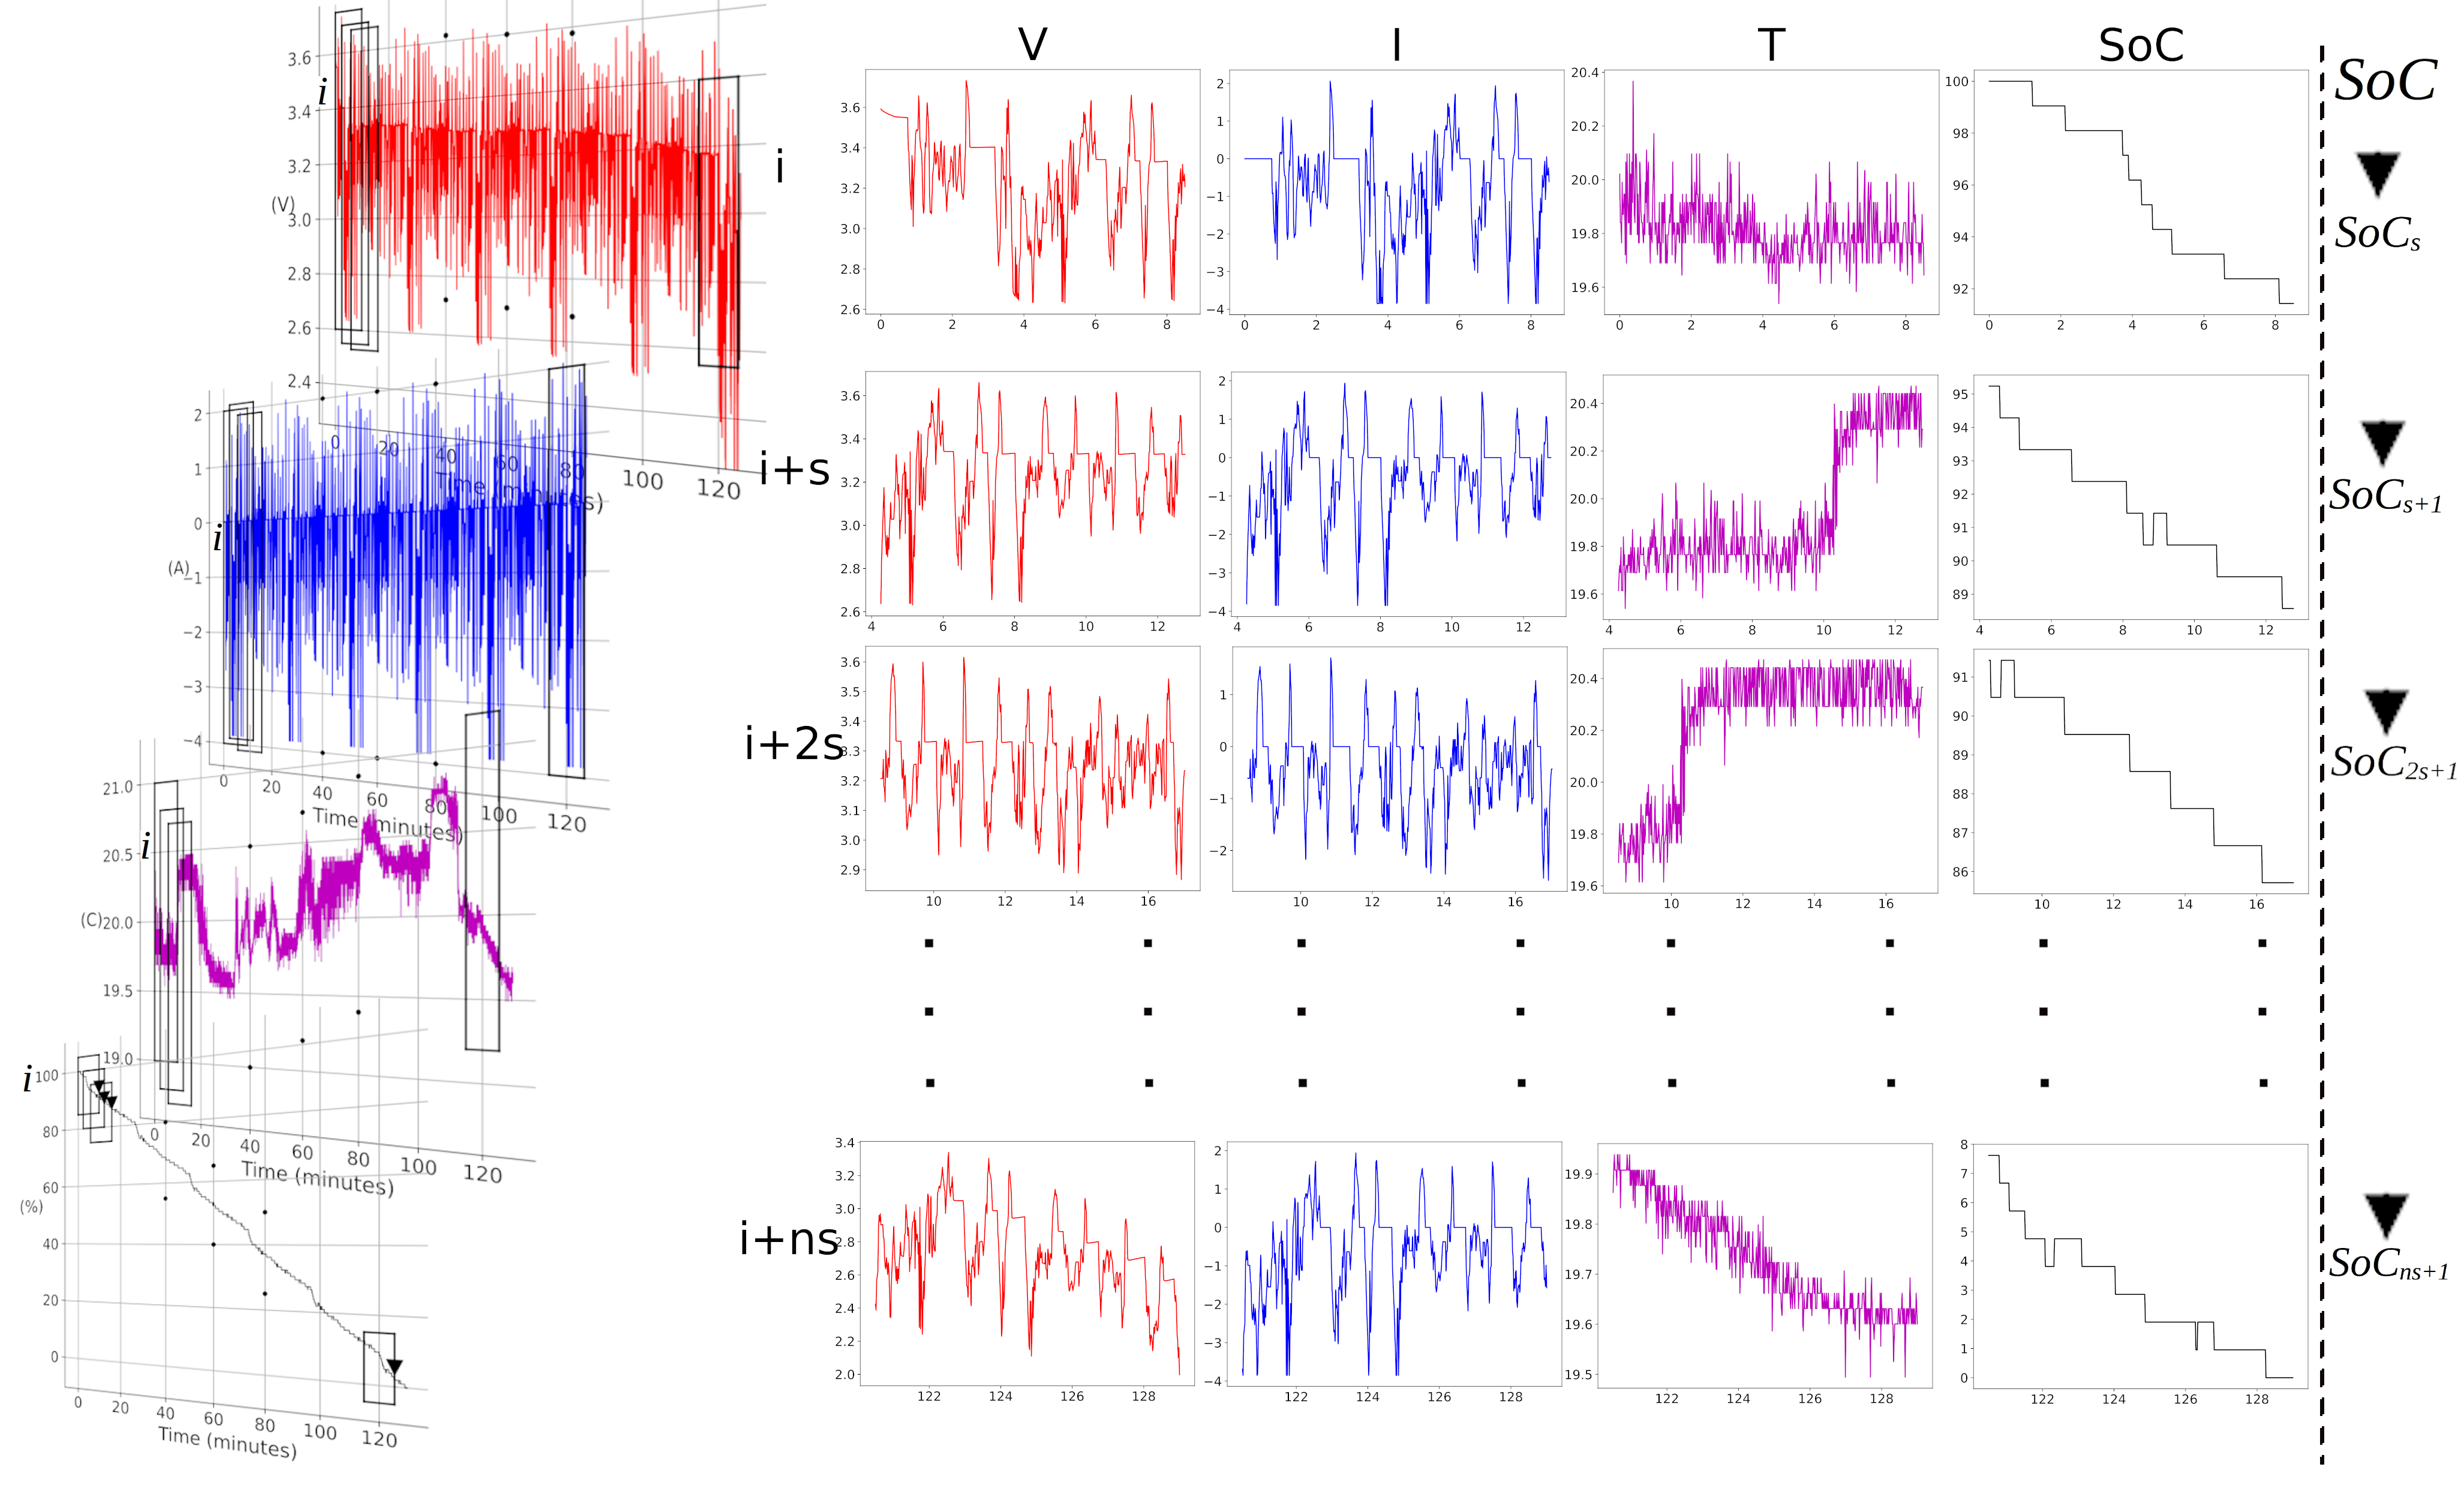
\includegraphics[width=0.9\linewidth]{II_Body/images/Windowing3D-1.jpg}
%         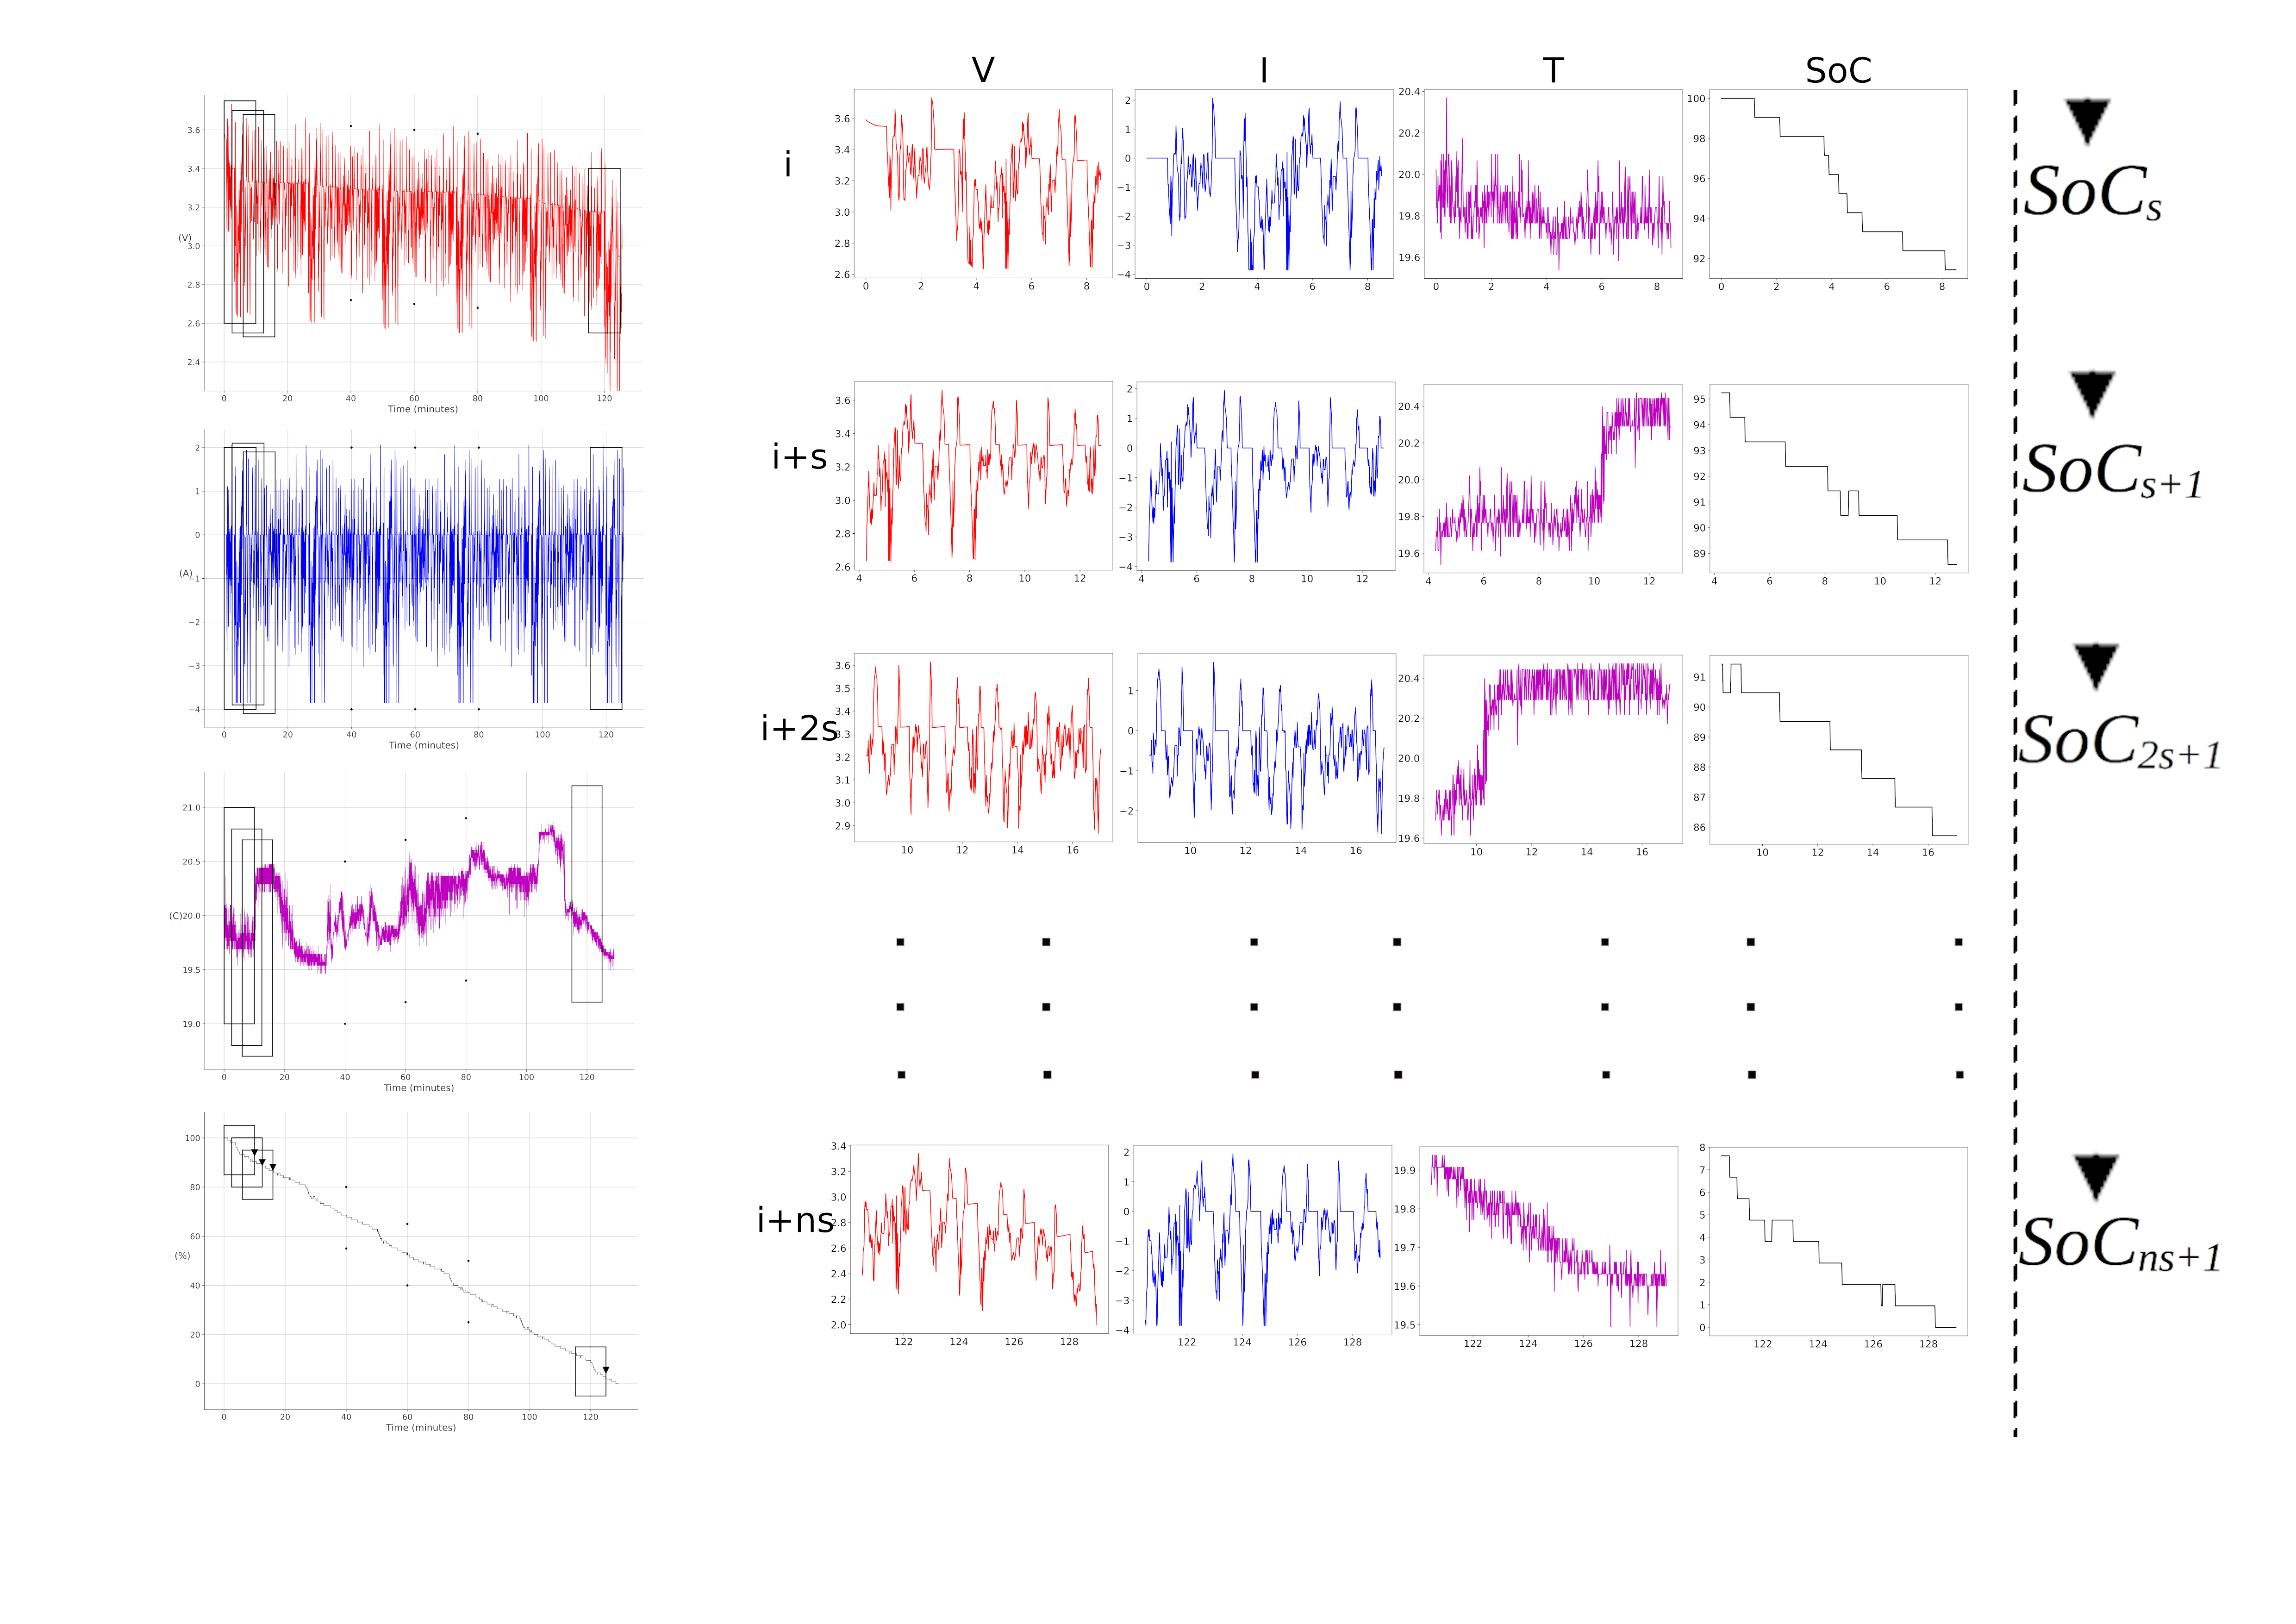
\includegraphics[width=0.9\linewidth]{II_Body/images/Windowing4f-A3.jpg}
%         \caption{Data Windowing scheme at 1Hz sampling rate with four features and one output. For visualisation purposes, the $s$-step has been used as 250 seconds, which is different from the actual implementation. The initial index $i$ was kept as a value close to the beginning of the data, around zero.}
%         \label{fig:Windowing}
%     \end{figure}
% \end{landscape}